\section{Бутстреп скользящих окон}

\noindent
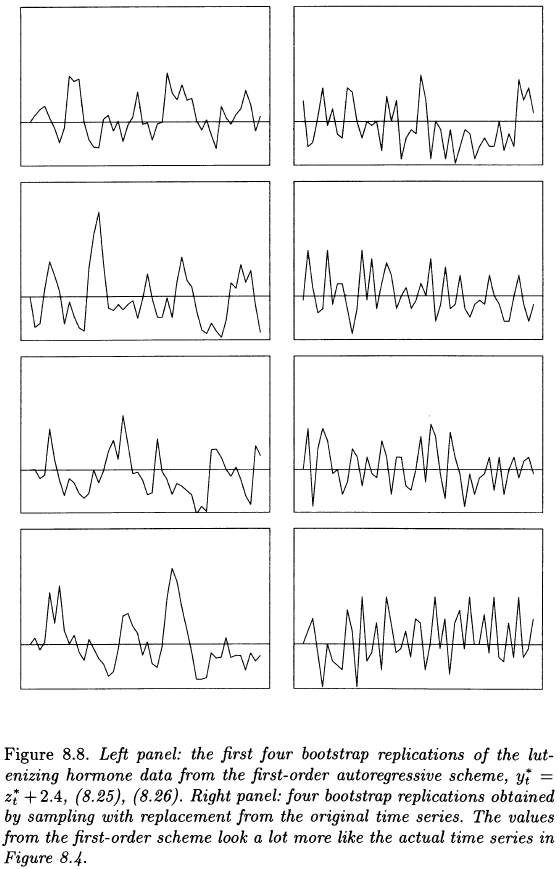
\includegraphics[width=\linewidth]{8/f88}
\newline

\noindent В этом разделе мы кратко опишем другой метод применения бутстрепа к временным рядам. Вместо подгонки модели и последующей выборки из остатков этот метод использует подход, более близкий к подходу, используемому для одновыборочных задач. Идея проиллюстрирована на рисунке 8.9. Исходный временной ряд представлен черными кружками. Чтобы сгенерировать бустреп реализацию временного ряда (белые кружки), мы выбираем длину окна («$3$» на диаграмме) и рассматриваем все возможные смежные окна этой длины. Мы составляем выборку с заменой из этих окон и объединяем их вместе, чтобы сформировать бутстреп временные ряды. Выбирается ровно столько окон, сколько необходимо для получения серии примерно такой же длины, что и исходная. Если длина окна равна $l$, то выберем $k$ окон так, чтобы $n \approx k \cdot l$.

Для иллюстрации мы выполним эти действия для данных о лютенизирующем гормоне. Интересующей статистикой была оценка $\hat \beta$ методом наименьших квадратов у AR(1). Мы выбрали длину окна $3$ и использовали бутстреп скользящих окон для генерации бустреп выборки для данных про лютенизирующий гормон. Типичная реализация бустрепа показана на рисунке 8.10, и она очень похожа на исходный временной ряд. Затем мы подогнали модель AR(1) к этому бутстреп временному ряду и оценили коэффициент $\hat \beta^*$ у AR(1). Весь этот процесс был повторен $B=200$ раз. (Обратите внимание, что модель AR(1) используется здесь для оценки $\beta$, но не используется при генерации бустреп реализаций временного ряда.) В результате стандартная ошибка бустрепа составила $\widehat {\text{se}}_{200} (\hat \beta) = 0.120$. Это примерно то же самое, что и значение $0.116$, полученное из AR(1) выборок, сгенерированных в предыдущем разделе. Увеличение размера окна до $5$ привело к уменьшению этого значения до $0.103$.

Чем оправдан бутстреп скользящих окон? Как мы видели ранее, мы не можем просто создать повторную выборку из отдельных наблюдений, так как это разрушило бы корреляцию, на которой мы хотим сфокусировать внимание. (Использование размера окна, равного единице, соответствует выборке с возвращением, и дает $0.139$ для оценки стандартной ошибки.) С бутстрепом скользящих окон идея состоит в том, чтобы выбрать размер окна $l$ достаточно большим, чтобы наблюдения, отстоящие более чем на $l$ единиц времени, были почти независимыми. Выбирая окна длиной $l$, мы сохраняем корреляцию, присутствующую в наблюдениях, отстоящих менее чем на $l$ единиц.

Бутстреп скользящих окон имеет то преимущество, что он менее «зависим от модели», чем подход бутстреп остатков, использовавшийся ранее. Как мы видели, последний метод зависит от модели, которая соответствует исходному временному ряду (например, модель AR(1) или AR(2)). Однако выбор размера окна $l$ может быть весьма важным, и эффективные методы для этого еще не разработаны.

В задаче регрессии, обсуждаемой в следующей главе, мы сталкиваемся с различными методами бустрепа, аналогичными подходам для временных рядов, которые мы обсуждали здесь.

\noindent
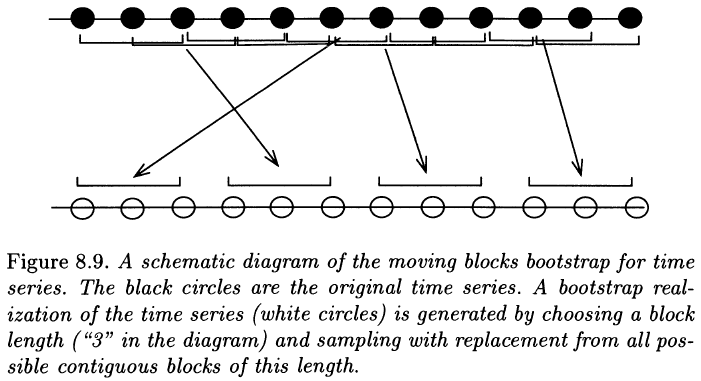
\includegraphics[width=\linewidth]{8/f89}
\newline

\noindent
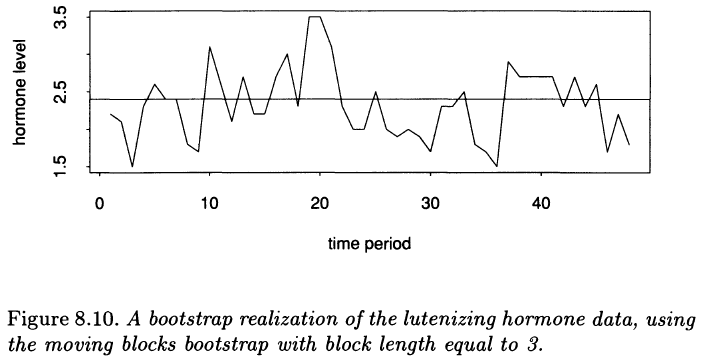
\includegraphics[width=\linewidth]{8/f810}
\newline